\documentclass[aspectratio=169]{beamer}
\usepackage{pgfpages}

% \setbeameroption{show only notes}
\setbeameroption{show notes}

% Handouts
% \pgfpagesuselayout{4 on 1}[letterpaper,border shrink=5mm,landscape]

% Presentation
% \pgfpagesuselayout{2 on 1}[a4paper,landscape]

\usetheme{PaperPlane}
% \usetheme{Darmstadt}


% Ensure one notes slide per content slide
\makeatletter
\def\beamer@framenotesbegin{
	\gdef\beamer@noteitems{}%
	\gdef\beamer@notes{{}}%
}
\makeatother

% Don't number the title slide
\let\otp\titlepage
\renewcommand{\titlepage}{\otp\addtocounter{framenumber}{-1}}

% Math operators
\DeclareMathOperator{\probability}{P}
\DeclareMathOperator{\expectedvalue}{E}


\title{A Generalized Probabilistic Gibbard-Satterthwaite Theorem}
\author{Jonathan Potter}
\institute[RIT]{Rochester Institute of Technology}

\begin{document}
	\begin{frame}[plain]
		\maketitle
	\end{frame}

	\section{Backround}

		\begin{frame}
			\frametitle{Importance of Elections}

			\begin{itemize}
				\item Political voting
				\item Electing board members
				\item Shareholders voting on company issues
				\item Artificial intelligent agent decision
				\item Search engine page-ranking
			\end{itemize}
		\end{frame}

		\begin{frame}
			\frametitle{Modeling an Election}

			\begin{itemize}
				\item Each voter ranks the alternatives (\emph{preference list})
				\item All the preference lists make up a \emph{preference profile}
				\item A \emph{voting rule} (election system, social choice function) chooses a winner based on a profile
			\end{itemize}

			\note{
				The interesting part is the voting rules.

				This field of study is called social choice theory.
			}
		\end{frame}

		\begin{frame}
			\frametitle{Fairness in Election Systems}

			\begin{itemize}
				\item Everyone should have an equal say
				\item Winner should accurately represent the group preference
				\item Simple with 2 alternatives; complicated with many
			\end{itemize}

			\note{
				With two alternatives the one preferred by the most voters should win.
			}
		\end{frame}

		\begin{frame}
			\frametitle{Manipulation}

			A voter can get a better result by voting strategically, rather than voting his actual preferences.

			\vspace{2em}
			\hspace*{1.2cm}{\Large Real Preferences}\hspace{5cm}{\Large Manipulation}

			\vspace{.5em}
			\centerline{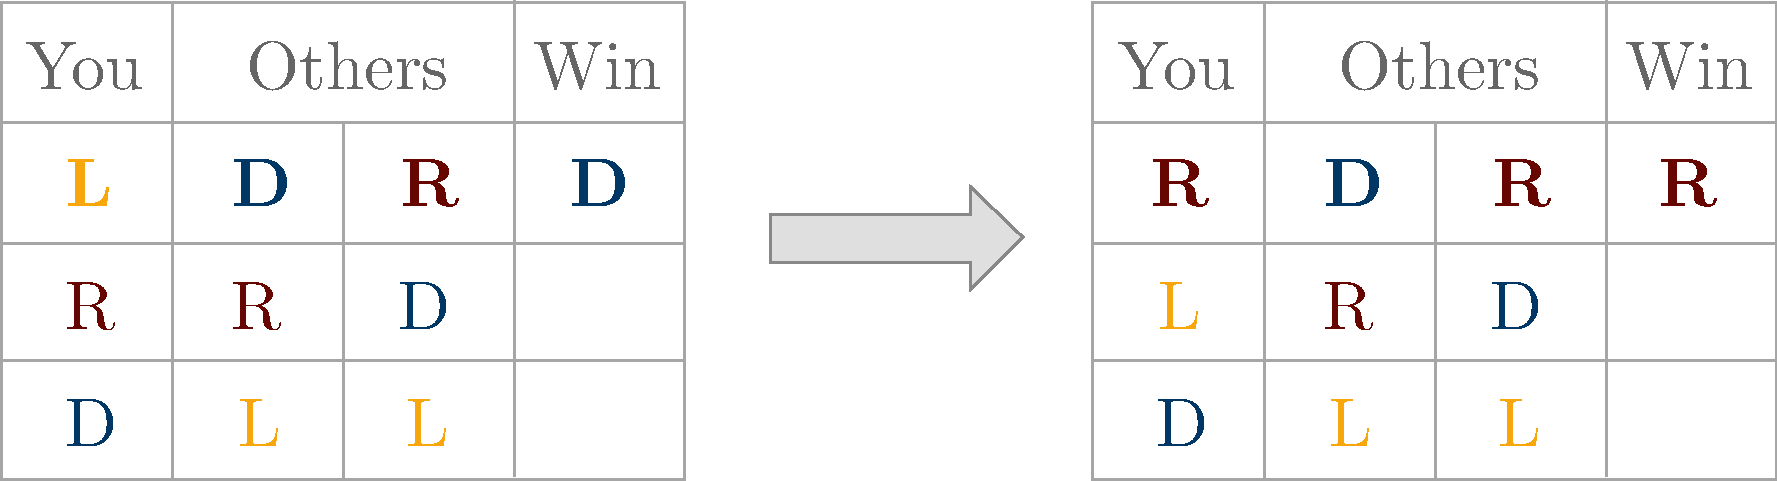
\includegraphics[height=0.4\paperheight, keepaspectratio]{../figures/manipulation_example.pdf}}

			\note{
				Manipulation is an enemy of fairness because the manipulative voter gets more influence than others.

				Assume a simple plurality/first-past-the-post system.

				In the first case it would be a tie, but lets assume our arbitrary tie breaking technique will choose the Democrats.

				This is essentially the ``wasted vote'' problem.

				This is a very simplistic example, but almost all voting systems are susceptible to manipulation.
			}
		\end{frame}

		\begin{frame}
			\frametitle{Gibbard-Satterthwaite Theorem}

			Voting rules are manipulable if they satisfy:

			\begin{description}
				\item[Non-dictatorship] No single voter always dictates the group preference.
				\item[Non-imposition] Every alternative has the possibility of winning.
			\end{description}

			\note{
				We would like to devise an unmanipulable voting rule, but this theorem says it's impossible.
			}
		\end{frame}

		\begin{frame}
			\frametitle{Circumventing the Gibbard-Satterthwaite Theorem}

			\begin{itemize}
				\item Searching for a computational barrier to manipulation
				\item Bartholdi, Tovey, and Trick studied the computational difficulty of finding a winner for various voting rules
				\item The Dodgson method is infeasible to manipulate because finding the winner is NP-hard
				\item Voting rules need to resist manipulation \emph{and} make it feasible to find the winner
			\end{itemize}

			\note{
				Many people have followed this line of research to great effect.
			}
		\end{frame}

		\begin{frame}
			\frametitle{Random Manipulation}

			\begin{itemize}
				\item Friedgut, Kalai, and Nisan studied random manipulation
				\item Succeeds with non-negligible probability
				\item Shows the limits of a computational barrier to manipulation
				\item Only proved results for elections with 3 alternatives
				\item This is the work I attempted to generalize
			\end{itemize}

			\note{
				If your alternative is not winning, randomly permute your preference list.
			}
		\end{frame}

		\begin{frame}
			\frametitle{Independent Work}
			\begin{itemize}
				\item Isaksson, Kindler, and Mossel have independently published a generalization in their paper \emph{The geometry of manipulation: A quantitative proof of the gibbard-satterthwaite theorem}
				\item They proved that for a neutral social choice function, a uniformly chosen profile will be manipulable with probability at least $2^{-1} \epsilon^2 n^{-4} m^{-6} (m!)^{-3}$
				\item Where $\epsilon$ is the distance from dictatorship
			\end{itemize}

			\note{
				As a disclaimer before a formal look at my work, others have published an independent generalization before I finished.

				This is unfortunate for me, but fortunate for the field of social choice theory as a whole.

				My work is still useful as:
				\begin{itemize}
					\item A simpler proof
					\item A proof that closely follows the original
					\item An alternative proof
				\end{itemize}
			}
		\end{frame}


	\section{Preliminaries}
	\subsection{Notation}

		\begin{frame}
			\frametitle{Notation}
			\begin{itemize}
				\item $C = \{1, \ldots, m\}$ is the set of alternatives.
				\item A preference list is a total ordering of the alternatives.
				\item The set of all preference lists is $L(C)$.
				\item A preference profile is a sequence of $n$ preference lists.
				\item The set of all preference profiles is $L(C)^n$.
				\item A voting rule is a function that chooses a winning alternative from a profile, i.e. $f : L(C)^n \to C$.
				\item An election is a voting rule paired with a profile: $(f, p)$.
			\end{itemize}

			\note{
				$L(C)^n$ is the Cartesian product of $L(C)$ with itself $n$ times, or the set of all $n$-tuples of elements of $L(C)$
			}
		\end{frame}

		\begin{frame}
			\frametitle{Restricted Preference Profiles}
			\begin{itemize}
				\item For a preference list $v$, $v|_D$ means $v$ \emph{restricted to} $D$, i.e. $v$ with the alternatives not in $D$ removed.
				\item For a preference profile, $p$, $p|_D$ means $p$ with each preference list restricted to $D$.
			\end{itemize}

			\hspace*{3.5cm}{\Large $p$}\hspace{6.2cm}{\Large $p|_{\{1, 2\}}$}

			\vspace{.5em}
			\centerline{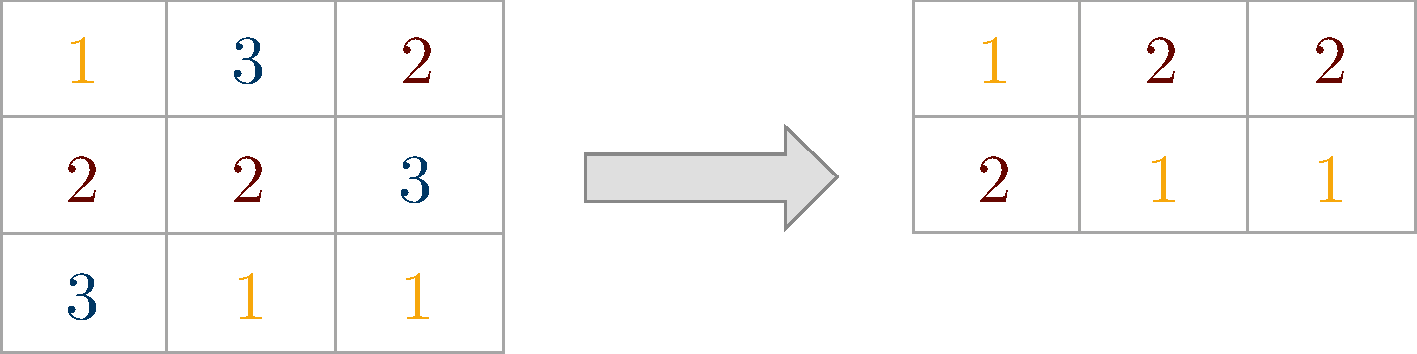
\includegraphics[height=0.3\paperheight, keepaspectratio]{../figures/restriction_example.pdf}}
		\end{frame}

		\begin{frame}
			\frametitle{Manipulation Power}

			\begin{itemize}
				\item Manipulation power $M_i(f)$, of voter $i$ on a social choice function $f$ is the probability that $p'_i$ is a profitable manipulation by voter $i$
				\item Where $p$ is a profile and $p'_i$ is a preference list which are both chosen uniformly at random
			\end{itemize}
		\end{frame}

		\begin{frame}
			\frametitle{Manipulation Potential}

			\[
				M^{a,b}(f) = \probability[f(p) = a, f(p') = b]
			\]

			\begin{itemize}
				\item Describes the scenario where all voters together attempt to manipulate $f$ to be $b$ rather than $a$
				\item $p$ and $p'$ are chosen uniformly at random
				\item Voters don't alter their preference between $a$ and $b$
			\end{itemize}

			\note{
				This definition does not require that anyone in particular gain from this, just that something ``unexpected'' happens.
			}
		\end{frame}


	\subsection{Proof Summary}

		\begin{frame}
			\frametitle{Proof Summary}

			Friedgut's proof is in three steps:

			\begin{description}
				\item[Step 1] Application of a quantitative version of Arrow's impossibility theorem.
				\item[Step 2] Reduction from an SCF with low dependence on irrelevant alternatives to a GSWF with a low paradox probability.
				\item[Step 3] Reduction from low manipulation power to low dependence on irrelevant alternatives.
			\end{description}
		\end{frame}

		\begin{frame}
			\frametitle{Generalized Steps}

			Friedgut, was able to generalize Step 1 and Step 2 as follows:

			\begin{lemma}[Generalized Step 1]
				For every fixed $m$ and $\epsilon > 0$ there exists $\delta > 0$ such that if $F = f^{\otimes \binom{m}{2}}$ is a neutral IIA GSWF over $m$ alternatives with $f : \{0,1\}^n \rightarrow \{0,1\}$, and $\Delta(f, DICT) > \epsilon$, then $F$ has probability of at least $\delta \ge (C\epsilon)^{\lfloor m/3 \rfloor}$ of not having a Generalized Condorcet Winner, where $C > 0$ is an absolute constant.
			\end{lemma}

			\begin{lemma}[Generalized Step 2]
				For every fixed $m$ there exists $\delta > 0$ such that for all $\epsilon > 0$ the following holds. Let $f$ be a neutral SCF among $m$ alternatives such that $\Delta(f, DICT) > \epsilon$. Then for all $(a,b)$ we have $M^{a,b}(f) \ge \delta$.
			\end{lemma}

			\note{
				So we only need to generalize step 3 to get the whole proof.
			}
		\end{frame}

		\begin{frame}
			\frametitle{Step 3}

			\begin{lemma}[Non-General Step 3]
				For every SCF $f$ on $3$ alternatives and every $a,b \in C$,
				\[
					M^{a,b}(f) \le \sum_i M_i(f) \cdot 6
				\]
			\end{lemma}

			\begin{lemma}[Generalized Step 3]
				For every SCF $f$ on $m$ alternatives and every $a,b \in C$,
				\[
					M^{a,b}(f) \le \sum_i M_i(f) \cdot m!
				\]
			\end{lemma}
		\end{frame}

		\begin{frame}
			\frametitle{Combining Steps}

			\begin{itemize}
				\item Step 3 is comprised of Lemma 6, Lemma 7, and Lemma 8 which we will generalize one at a time
				\item When we put together all 3 generalized steps we get our main result
			\end{itemize}
		\end{frame}

	\section{Results}
	\subsection{Lemma 6}

		\begin{frame}
			\frametitle{Statement of Lemma 6}

			\begin{lemma}[Original Lemma 6]
				\[
					M^{a,b}(f) = \expectedvalue_{p} \left[ \frac{|A(p)|}{3^n} \cdot \frac{|B(p)|}{3^n} \right],
				\]
				where $p \in L(C)^n$ is chosen uniformly at random.
			\end{lemma}

			\begin{lemma}[Generalized Lemma 6]
				\[
					M^{a,b}(f) = \expectedvalue_{p} \left[ \frac{|A(p)|}{\left(\frac{m!}{2}\right)^n} \cdot \frac{|B(p)|}{\left(\frac{m!}{2}\right)^n} \right],
				\]
				where $p \in L(C)^n$ is chosen uniformly at random.
			\end{lemma}
		\end{frame}

		\begin{frame}
			\frametitle{Define $A$ and $B$ Functions}

			Let $a, b \in C$ be the first two alternatives, let $p \in L(C)^n$ be a preference profile. We define
			\begin{align*}
				A(p) &= \{x \in L(C)^n \mid x|_{\{a,b\}} = p|_{\{a,b\}}, f(x) = a\} \\
				B(p) &= \{x \in L(C)^n \mid x|_{\{a,b\}} = p|_{\{a,b\}}, f(x) = b\}.
			\end{align*}
		\end{frame}

		\begin{frame}
			\frametitle{Recall $M^{a,b}$ Definition}

			Recall the definition of $M^{a,b}(f)$:
			\[
				M^{a,b}(f) = \probability[f(p) = a, f(p') = b]
			\]
			where $p, p'$ are chosen at random in $L(C)^n$ with $p|_{\{a,b\}} = p'|_{\{a,b\}}$.
		\end{frame}

		\begin{frame}
			\frametitle{Size of Profiles}

			For any preference profile $p \in L(C)^n$ there are $(\frac{m!}{2})^n$ profiles $x$ such that $x|_{\{a, b\}} = p|_{\{a, b\}}$ because:

			\begin{itemize}
				\item There are $m!$ possible preference lists
				\item Half of them will have the preference between $a$ and $b$ that agrees with $p_i|_{\{a, b\}}$, for any $i$
				\item This gives $\frac{m!}{2}$ possible preference lists for each voter
				\item So there are $(\frac{m!}{2})^n$ profiles comprised of these preference lists
			\end{itemize}
		\end{frame}

		\begin{frame}
			\frametitle{Proof of Generalized Lemma 6}

			\begin{itemize}
				\item First we fix a profile $q$
				\item There are $(\frac{m!}{2})^n$ profiles that agree with $q|_{\{a,b\}}$
				\item $|A(q)|$ is the number of those for which the outcome is $a$
				\item Randomly choose a profile, $p$, satisfying $p|_{\{a,b\}} = q|_{\{a,b\}}$
				\item So the probability that $f(p) = a$ is
					\[
						\frac{|A(q)|}{\left(\frac{m!}{2}\right)^n}
					\]
			\end{itemize}
		\end{frame}

		\begin{frame}
			\frametitle{Proof of Generalized Lemma 6}

			\begin{itemize}
				\item Likewise, randomly choose a profile, $p'$, satisfying $p'|_{\{a,b\}} = q|_{\{a,b\}}$
				\item And the probability that $f(p') = b$ is
					\[
						\frac{|B(q)|}{\left(\frac{m!}{2}\right)^n}
					\]
			\end{itemize}
		\end{frame}

		\begin{frame}
			\frametitle{Proof of Generalized Lemma 6}

			Since $p|_{\{a,b\}} = q|_{\{a,b\}}$ and $p'|_{\{a,b\}} = q|_{\{a,b\}}$, clearly we have that $p|_{\{a,b\}} = p'|_{\{a,b\}}$. Since $f(p) = a$ and $f(p') = b$ are independent events, the joint probability is
			\[
				\frac{|A(q)|}{\left(\frac{m!}{2}\right)^n} \cdot \frac{|B(q)|}{\left(\frac{m!}{2}\right)^n}.
			\]
		\end{frame}

		\begin{frame}
			\frametitle{Proof of Generalized Lemma 6}

			So we can rewrite
			\[
				M^{a,b}(f) = \probability[f(p) = a, f(p') = b]
			\]
			as
			\[
				M^{a,b}(f) = \expectedvalue_{q} \left[ \frac{|A(q)|}{\left(\frac{m!}{2}\right)^n} \cdot \frac{|B(q)|}{\left(\frac{m!}{2}\right)^n} \right],
			\]
			\qed
		\end{frame}


	\subsection{Lemma 7}

		\begin{frame}
			\frametitle{Statement of Lemma 7}

			\begin{lemma}[Original Lemma 7]
				\[
					\sum_i M_i(f) \ge \frac{1}{6} 3^{-n} \expectedvalue_p \left[|\partial A(p)| + |\partial B(p)| \right]
				\]
			\end{lemma}

			\begin{lemma}[Generalized Lemma 7]
				\[
					\sum_i M_i(f) \ge \frac{1}{m!} \left(\frac{m!}{2}\right)^{-n} \expectedvalue_p \left[|\partial A(p)| + |\partial B(p)| \right]
				\]
			\end{lemma}
		\end{frame}

		\begin{frame}
			\frametitle{Profile Lattice}

			\centerline{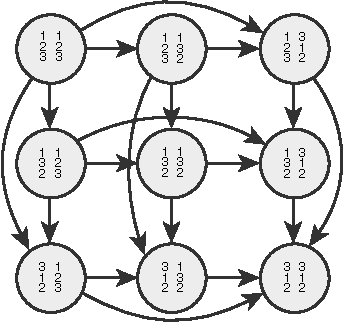
\includegraphics[height=0.7\paperheight, keepaspectratio]{../figures/profile_lattice.pdf}}
		\end{frame}

		\begin{frame}
			\frametitle{Upper Edge Border}

			\begin{columns}
				\begin{column}{0.5\textwidth}
					\begin{itemize}
						\item Set of edges whose tail is in $A(p)$ and whose head is not in $A(p)$
						\item Denoted $\partial A(p)$
						\item Edge notation: $(x_{-i}, x_i, x'_i)$ as shorthand for $((x_{-i},x_i), (x_{-i},x'_i))$
					\end{itemize}
				\end{column}

				\begin{column}{0.5\textwidth}
					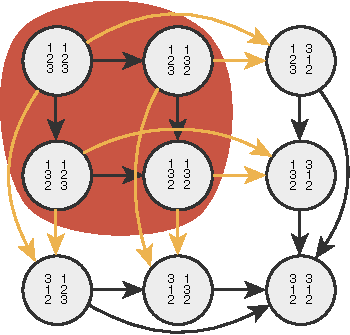
\includegraphics[height=0.7\paperheight, keepaspectratio]{../figures/profile_lattice_edge_border.pdf}
				\end{column}
			\end{columns}

			\note{
				$x_{-i}$ is $x$ without the $i$th index.
			}
		\end{frame}

		\begin{frame}
			\frametitle{Formal Definition of Upper Edge Border}

			\begin{alignat*}{4}
				\partial_i A(p) &= \{ (x_{-i}, x_i, x'_i) \mid \hspace{1mm} & (x_{-i}, x_i) &\in A(p), \\
				&& (x_{-i}, x'_i) &\notin A(p), \\
				&& x_i|_{\{a,b\}} &= x'_i|_{\{a,b\}}, \\
				&& x_i &<_s x'_i \} \\
				\partial A(p) &= \bigcup_j \partial_j A(p) &&
			\end{alignat*}

			\note{
				We don't have time to go into more of the lattice work I've done, including $<_s$.

				$<_s$ means something like being close to the $(1, 2, 3)$ ordering.

				We define the upper edge border of $B(p)$ analogously.
			}
		\end{frame}

		\begin{frame}
			\frametitle{Edges Correspond to Manipulations}

			\begin{lemma}
				Each $(x_{-i}, x_i, x'_i) \in \partial_i A(p) \cup \partial_i B(p)$ corresponds to at least one successful manipulation.
			\end{lemma}

			\note{
				We don't have time to show the proof, but it's in my paper.
			}
		\end{frame}

		\begin{frame}
			\frametitle{Proof of Generalized Lemma 7}

			\begin{itemize}
				\item Randomly choose $p$ and $p'_i$
				\item $M_i(f)$ is the probability that $p'_i$ is a successful manipulation
				\item We wish to come up with a lower bound for $M_i(f)$
				\item We can think of these as two distinct profiles, $p$ and $p'$, where $p' = (p_{-i}, p'_i)$
				\item Clearly $p_{-i}|_{\{a,b\}} = p'_{-i}|_{\{a,b\}}$
				\item We have $p_i|_{\{a,b\}} = p'_i|_{\{a,b\}}$ with probability $\frac{1}{2}$, and we condition the following on this being the case
				\item So $p|_{\{a,b\}} = p'|_{\{a,b\}}$
			\end{itemize}
		\end{frame}

		\begin{frame}
			\frametitle{Proof of Generalized Lemma 7}

			\begin{itemize}
				\item Since every edge in $\partial_i A(p) \cup \partial_i B(p)$ corresponds to at least one manipulation, we can lower bound $M_i(f)$ by the probability that an edge is in $\partial_i A(p) \cup \partial_i B(p)$
				\item The total number of possible edges of the form $(x_{-i}, x_i, x'_i)$ is
					\[
						(m!)^{n-1} \cdot m! \cdot m!
					\]
				\item But all edges in $\partial_i A(p) \cup \partial_i B(p)$ must agree with $p|_{\{a, b\}}$. The total number of possible edges agreeing with $p|_{\{a, b\}}$ is
					\[
						\left(\frac{m!}{2}\right)^{n-1} \cdot \frac{m!}{2} \cdot \frac{m!}{2} = \frac{m!}{2}\left(\frac{m!}{2}\right)^{n}
					\]
				\item Since $\partial_i A(p)$ and $\partial_i B(p)$ are disjoint, no edge can be in both sets and so we have
					\[
						|\partial_i A(p) \cup \partial_i B(p)| \le \frac{m!}{2}\left(\frac{m!}{2}\right)^{n}
					\]
			\end{itemize}
		\end{frame}

		\begin{frame}
			\frametitle{Proof of Generalized Lemma 7}

			\begin{itemize}
				\item Therefore, the probability that a randomly chosen edge is in either $\partial_i A(p)$ or $\partial_i B(p)$ is
					\[
						\frac{2}{m!} \left(\frac{2}{m!}\right)^{n} \cdot \expectedvalue_p \left[ |\partial_i A(p)| + |\partial_i B(p)| \right]
					\]
				\item We conditioned our analysis on $p_{-i}|_{\{a,b\}} = p'_{-i}|_{\{a,b\}}$, so our lower bound becomes
					\[
						M_i(f) \ge \frac{1}{2} \cdot \frac{2}{m!}\left(\frac{2}{m!}\right)^{n} \cdot \expectedvalue_p \left[ |\partial_i A(p)| + |\partial_i B(p)| \right].
					\]
			\end{itemize}
		\end{frame}

		\begin{frame}
			\frametitle{Proof of Generalized Lemma 7}

			\begin{itemize}
				\item Simplifying gives
					\[
						M_i(f) \ge \frac{1}{m!}\left(\frac{2}{m!}\right)^{n} \cdot \expectedvalue_p \left[ |\partial_i A(p)| + |\partial_i B(p)| \right].
					\]
				\item Summing over $i$ gives
					\[
						\sum_i M_i(f) \ge \frac{1}{m!}\left(\frac{2}{m!}\right)^{n} \cdot \expectedvalue_p \left[ |\partial A(p)| + |\partial B(p)| \right].
					\]
			\end{itemize}

			\qed
		\end{frame}


	\subsection{Lemma 8}

		\begin{frame}
			\frametitle{Lemma 8}

			\begin{lemma}[Original Lemma 8]
				\[
					|\partial A(p)| + |\partial B(p)| \ge \left( \frac{1}{3} \right)^n |A(p)| \cdot |B(p)|
				\]
			\end{lemma}

			\begin{lemma}[Generalized Lemma 8]
				\[
					|\partial A(p)| + |\partial B(p)| \ge \left( \frac{2}{m!} \right)^n |A(p)| \cdot |B(p)|
				\]
			\end{lemma}

			\note{
				I got close, but wasn't able to complete the proof of this lemma.

				In my thesis I give a partial proof and a detailed description of the things that would be required to make it work.

				Because of lack of time, I won't go into it here.
			}
		\end{frame}


	\subsection{Step 3}
		\begin{frame}
			\frametitle{Combining Lemma 6, 7, and 8}

			Restatement of the lemmas:
			\begin{align*}
				&M^{a,b} = \expectedvalue[|A||B|] \cdot L_6 & \textrm{lemma 6} \\
				&L_7 \cdot \expectedvalue[|\partial A| + |\partial B|] \le \sum_i M_i & \textrm{lemma 7} \\
				&\frac{1}{L_8} \cdot (|\partial A| + |\partial B|) \ge |A||B| & \textrm{lemma 8}
			\end{align*}

			Now we can solve for the result of step 3:
			\begin{align*}
				M^{a,b} &= \expectedvalue[|A||B|] \cdot L_6 & \textrm{lemma 6} \\
				M^{a,b} &\le \expectedvalue[|\partial A| + |\partial B|] \cdot \frac{L_6}{L_8} & \textrm{by lemma 8} \\
				M^{a,b} &\le \sum_i M_i \cdot \frac{L_6}{L_7L_8} & \textrm{by lemma 7}
			\end{align*}

			\note{
				Because it's \emph{much} easier to read:
				\begin{itemize}
					\item $A \equiv A(p)$
					\item $M^{a,b} \equiv M^{a,b}(f)$
					\item $M_i \equiv M_i(f)$
				\end{itemize}
			}
		\end{frame}

		\begin{frame}
			\frametitle{Combining Lemma 6, 7, and 8}

			The variables have the following values:
			\begin{align*}
				L_6 &= \left(\frac{m!}{2}\right)^{-2n} \\
				L_7 &= \frac{1}{m!}\left(\frac{m!}{2}\right)^{-n} \\
				L_8 &= \left(\frac{m!}{2}\right)^{-n}
			\end{align*}

			Substituting becomes:
			\begin{align*}
				\frac{L_6}{L_7L_8} &= \left(\frac{m!}{2}\right)^{-2n} \cdot m!\left(\frac{m!}{2}\right)^{n} \cdot \left(\frac{m!}{2}\right)^{n} \\
				&= \left(\frac{m!}{2}\right)^{-2n} \cdot m! \cdot \left(\frac{m!}{2}\right)^{2n} \\
				&= m!
			\end{align*}
		\end{frame}

		\begin{frame}
			\frametitle{Step 3 Result}

			The final result for step 3 is:
			\[
				M^{a,b}(f) \le \sum_i M_i(f) \cdot m!
			\]

			By combining it with Friedgut's step 1 and 2 we get the generalized main theorem:
			\begin{theorem}[Main Result]
				There exists a constant $C > 0$ such that for every $\epsilon > 0$ the following holds. If $f$ is a neutral SCF for $n$ voters over $m$ alternatives and $\Delta(f, g) > \epsilon$ for any dictatorship $g$, then $f$ has total manipulatiblity:
				\[
					\sum^n_{i=1} M_i(f) \ge \frac{(C\epsilon)^{\lfloor m/3 \rfloor}}{m!}.
				\]
			\end{theorem}

			\note{
				In this case $C$ is a constant, and not the set of the alternatives.
			}
		\end{frame}


	\section{Questions}

		\begin{frame}
			\frametitle{Questions}

			\vspace*{-0.12cm}
			\centerline{
\includegraphics[height=0.85\paperheight, keepaspectratio]{../figures/question_kitten.jpg}}
		\end{frame}
\end{document}
